\documentclass[a4paper]{article}
\usepackage[utf8]{inputenc}
\usepackage[T1]{fontenc}
\usepackage[intlimits]{amsmath}
\usepackage{amsfonts}
\usepackage{amssymb}
\usepackage[export]{adjustbox}
\usepackage{graphicx}
\setlength{\parindent}{0pt}
\usepackage[left=1in, right=1in, top=1in, bottom=1in]{geometry}
\usepackage{float}
\usepackage{multicol}
\usepackage{listings}
\usepackage{xcolor}
\usepackage{cancel}
\usepackage{bm}
\usepackage{hyperref}
\setcounter{tocdepth}{1}
\usepackage[titletoc]{appendix}
\hypersetup{
	colorlinks=true,
	linkcolor=blue,
	filecolor=blue,
	urlcolor=blue,
}

\newcommand\blfootnote[1]{%
	\begingroup
	\renewcommand\thefootnote{}\footnote{#1}%
	\addtocounter{footnote}{-1}%
	\endgroup
}

\begin{document}
	
	\Huge\textbf{Projectile Trajectory Calculator}
	\newline
	\LARGE AMB Calculator
	
	\vspace{0.5cm}
	\normalsize
	
	This calculator is used to help plan the trajectory of an object launched by a shooter. It can be used both to predict the object's final position and heading angle based on the initial values, or to calculate the needed initial values to arrive at the desired target values. All angles are measured in degrees above the horizontal.
	
	
	\section*{Find Target Values}
	
	These modes iteratively simulates the object's trajectory from its launch until it hits the target, defined either by a horizontal distance or both a vertical height and direction of travel. In this mode, the simulation can incorporate drag and lift (Magnus) forces for spherical objects. In this configuration we will refer to the spherical object as a ball, but the purely parabolic equations hold for objects of any shape by setting the respective coefficients to zero.\\
	
	We have a ball of radius $ r $ and mass $ m $, moving at velocity $ \bar{v} $ with rotational velocity $ \bar{\omega} $. The ball has cross-sectional area $ A_c = \pi r^2 $, and drag and lift coefficients $ C_D $ and $ C_L $ respectively. At any time $ t $ there are three forces acting on the ball: the gravity force $ F_g $, drag force $ F_D $, and lift force $ F_L $. These can be expressed in vector form as:
	
	\begin{equation}
		F_g = m g \left( - \hat{y} \right)
	\end{equation}
	
	\begin{equation}
		F_D = \frac{1}{2} \rho \left| \bar{v} \right|^2 A_c C_D \left( - \hat{v} \right)
		= \frac{\pi}{2} \rho r^2 v^2 C_D \left( -\hat{v} \right)
	\end{equation}
	
	\begin{equation}
		F_L = \frac{1}{2} \rho \left| \bar{v} \right|^2 A_c C_L \left( \hat{\omega} \times \hat{v} \right)
		= \frac{\pi}{2} \rho r^2 v^2 C_L \left( \hat{\omega} \times \hat{v} \right)
	\end{equation}
	\\
	where $ \rho $ is the air density and $ g $ is the gravitational constant.\\
	
	We will define $ \theta_v $ as the angle of $ \hat{v} $ counter-clockwise relative to $ + \hat{x} $. So we can combine the $ x $ and $ y $ components of all the forces:
	
	\begin{gather}
	\begin{aligned}
		m a_x = \sum F_x &= -F_L \sin \theta_v - F_D \cos \theta_v \\
		&= - \frac{\pi}{2} \rho r^2 v^2 \left( C_L \sin \theta_v + C_D \cos \theta_v \right) \\
		&= - \frac{\pi}{2} \rho r^2 v \left( C_L \cdot v_y + C_D \cdot v_x \right)
	\end{aligned}
	\end{gather}
	
	\begin{gather}
		\begin{aligned}
			m a_y = \sum F_y &= F_L \cos \theta_v - F_D \sin \theta_v - F_g \\
			&= \frac{\pi}{2} \rho r^2 v^2 \left( C_L \cos \theta_v - C_D \sin \theta_v \right) - mg \\
			&= \frac{\pi}{2} \rho r^2 v \left( C_L \cdot v_x - C_D \cdot v_y \right) - mg
		\end{aligned}
	\end{gather}
	\\
	Starting with $ \bar{x} = \bar{0} $ and $ \bar{v} = v_i \angle \theta_i $, we can calculate the acceleration components $ a_x $ and $ a_y $. We can then calculate the position and velocity of the ball at the next timestep as:
	
	\begin{equation}
		\bar{v}_{i+1} = \bar{v}_i + \bar{a} \cdot dt \qquad\implies\qquad
		\bar{x}_{i+1} = \bar{x}_{i} + \bar{v}_i \cdot dt + \tfrac{1}{2} \bar{a} \cdot dt^2		
	\end{equation}
	
	\newpage
	The simulation end condition is determined by the mode. For "Find Target Values by Target Distance", the simulation ends when $ x_x \geq d $, the horizontal distance to the target. For "Find Target Values by Target Height", the simulation ends when $ x_y \geq h_{target} $ and $ v_y \leq 0 $ if the target height direction arrow is up, or $ x_y \leq h_{target} $ and $ v_y \leq 0 $ if the target direction arrow is down.\\
	
	If drag and Magnus forces are ignored, we can use traditional parabolic trajectory equations to find the object's final position and angle:
	
	\begin{gather}
	\begin{aligned}
		h_{target} &= h_0 + d \cdot \tan \theta_0 - \frac{g \cdot d^2}{2 v_0^2 \cos^2 \theta_0} \iff \\
		d &= \frac{v_0^2 \cos^2 \theta_0}{g} \left( \tan \theta_0 \pm \sqrt{\tan^2 \theta_0 - \frac{2g}{v_0^2 \cos^2 \theta_0} \left( h_{target} - h_0 \right) } \right)
	\end{aligned}
	\end{gather}
	
	\begin{equation}
		\theta_{target} = \tan^{-1} \left( 2\ \frac{h_{target} - h_0}{d} - \tan \theta_0 \right)
	\end{equation}
	
	
	\section*{Find Launch Values}
	
	This mode calculates the launch velocity and angle needed to arrive at the desired target values in the absence of drag or Magnus forces. //
	
	Starting with basic projectile motion equations:
	
	\begin{equation} \label{Dx}
		\Delta x = v_0 \cos \theta_0 \cdot t
	\end{equation}
	
	\begin{equation} \label{Dy}
		\Delta y = v_0 \sin \theta_0 \cdot t - \tfrac{1}{2} g \cdot t^2
	\end{equation}
	
	\begin{equation} \label{th_target}
		\theta_{target} = \tan^{-1} \left( \frac{v_{y, target}}{v_{x, target}} \right) = \tan^{-1} \left( \frac{v_0 \sin \theta_0 - g \cdot t}{v_0 \cos \theta_0} \right)
	\end{equation}
	\\
	Solving (\ref{Dx}) for $ t $ and substituting into (\ref{Dy}) gives:
	
	\begin{equation}
		\Delta y = \Delta x \cdot \tan \theta_0 - \frac{g \cdot \left( \Delta x \right)^2}{2 v_0^2 \cos^2 \theta_0}
	\end{equation}
	\\
	And with $ \Delta x = d $ and $ \Delta y = h_{target} - h_0 $:
	
	\begin{equation} \label{hf}
		h_{target} = h_0 + d \cdot \tan \theta_0 - \frac{g \cdot d^2}{2 v_0^2 \cos^2 \theta_0}
	\end{equation}
	\\
	Substituting $ t $ from (\ref{Dx}) into (\ref{th_target}):
	
	\begin{equation}
		\theta_{target} = \tan^{-1} \left( \frac{v_0 \sin \theta_0 - g \cdot \frac{\Delta x}{v_0 \cos \theta_0}}{v_0 \cos \theta_0} \right)
		 = \tan^{-1} \left( \tan \theta_0 - \frac{g \cdot d}{v_0^2 \cos^2 \theta_0} \right)
	\end{equation}
	\\
	Further substituting in (\ref{hf}) and simplifying gives:
	
	\begin{equation}
		\theta_{target} = \tan^{-1} \left( 2 \frac{h_{target} - h_0}{d} - \tan \theta_0 \right)
	\end{equation}
	\\
	Which can easily be solved for $ \theta_0 $:
	
	\begin{equation}
		\theta_0 = \tan^{-1} \left( 2 \frac{h_{target} - h_0}{d} - \tan \theta_{target} \right)
	\end{equation}
	
	\newpage
	We can then substitute in (\ref{hf}):
	
	\begin{equation}
		\tan \theta_{target} - \tan \theta_0 = - \frac{g \cdot d}{v_0^2 \cos^2 \theta_0}
	\end{equation}
	\\
	Which can be solved for $ v_0 $:
	
	\begin{equation}
		v_0 = \sec \theta_0 \cdot \sqrt{\frac{g \cdot d}{\left| \tan \theta_{target} - \tan \theta_0 \right|}}
	\end{equation}
	\\
	Thus we have the initial velocity $ v_0 $ and angle $ \theta_0 $. We can then run the simulator without drag or Magnus forces to track the projectile's trajectory.\\
	
	
	\section*{Experimentally Determining Drag and Lift Coeffieicnts}
	
	For the lift coefficient, we can use experiments done at the University of Illinois. They defined a dimensionless quantity called the spin factor, $ s = \frac{r \cdot \omega}{v} $, based on the ball's rotational and linear velocities $ \omega $ and $ v $. They found that the lift coefficient is directly related to this parameter, following $ C_L = 1.6 s $ for $ s < 0.1 $ and $ C_L = 0.6 s + 0.1 $ for $ s > 0.1 $. By entering the rotational velocity, assumed to be constant throughout the trajectory, the simulation automatically calculates the lift coefficient according to the spin factor for each timestep.\\
	
	Determining the drag coefficient is more complicated. Earlier versions calculated the Reynolds number of the ball and used that to find the drag coefficient, but this method was not very accurate as typical values often fell in the transition range between laminar and turbulent flow. Instead, the recommended method now involves experimental testing by dropping the ball off a high surface of known height and measuring the time it takes to hit the ground.\\
	
	We will define a constant $ \alpha = \frac{\pi}{2 m} \rho r^2 C_D  $. In this case, the motion equation is:
	
	\begin{equation}
		m a = m \frac{dv}{dt} = \sum F = F_D - F_g = \alpha m v^2 (t) - m g
	\end{equation}
	\\
	This differential equation can be solved for $ v(t) $ with initial condition $ v(0) = 0 $:
	
	\begin{equation}
		v(t) = -\sqrt{\frac{g}{\alpha}} \tanh \left( \sqrt{\alpha g} \cdot t \right)
	\end{equation}
	\\
	This can then be integrated with initial condition $ x(0) = h $ to get the position equation:
	
	\begin{equation}
		x(t) = h - \frac{1}{\alpha} \ln \left( \cosh \left( \sqrt{g \alpha} \cdot t \right) \right)
	\end{equation}
	\\
	So solving for the time the ball hits the ground, $ x(t) = 0 $, gives:
	
	\begin{equation}
		t = \frac{1}{\sqrt{g \alpha}} \cosh^{-1} \left( \exp \left( \alpha \cdot h \right) \right)
	\end{equation}
	
	\newpage
	We would like to solve for $ \alpha $ in order to find $ C_D $, but unfortunately this is not possible to do analytically. Instead, we will use the following graph to find $ \alpha $ based on the drop height $ h $ (in meters) and the time the ball takes to hit the ground:
	
	\begin{figure}[H]
		\centering
		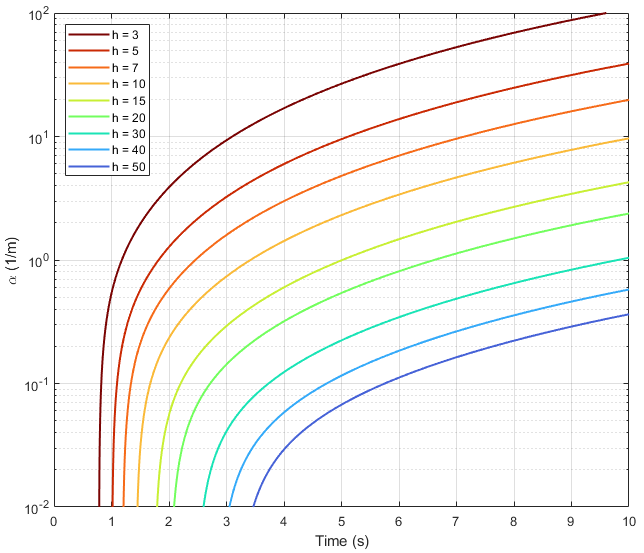
\includegraphics[width=\linewidth]{projectile_drag}
	\end{figure}
	
	We can now find $ C_D $ using the definition of $ \alpha $:
	
	\begin{equation}
		C_D = \frac{2\alpha \cdot m}{\pi \rho \cdot r^2}
	\end{equation}
	\\
	Where $ m $ is the ball's mass, $ r $ is its radius, and $ \rho $ is the density of air ($ 1.275\ \frac{\text{kg}}{\text{m}^3} $ at STP). Note that all of the units in the equation should match so that $ C_D $ is a dimensionless parameter.
	
	
	\blfootnote{The equations in this calculator are based in part by work done by the \href{http://baseball.physics.illinois.edu/ajpfeb08.pdf}{University of Illinois Department of Physics}}
	
	
	
\end{document}